\begin{frame}
	\myheading{Module 13.8 : Deep Dream}
\end{frame}

%%%%%%%%%%%%%%%%%%%%%%%%%%%%%%%%%%%%%%%%%%%%%%%%%%%%%%%%%%%%%%%%%%%%%%%%%%%%%%%%%%%%%%%%%

\begin{frame}
	\begin{columns}
		\column{0.5\textwidth}	
		
		\begin{overlayarea}{\textwidth}{\textheight}
			\begin{tikzpicture}
				
				\onslide<1->{
					\node[inner sep=0pt] (B) at (-4.7,12.5){
					%\begin{center}
\begin{tikzpicture}[scale=0.4,transform shape]

\pgfsetxvec{\pgfpoint{1cm}{0cm}}
\pgfsetyvec{\pgfpoint{0cm}{1cm}}
\pgfsetzvec{\pgfpoint{-.5cm}{-.866cm}}

\def\cuboid#1#2#3#4#5{
\begin{scope}
\edef\mycolor{#2}
\edef\depth{#3}
\edef\height{#4}
\edef\width{#5}
\draw[black,fill=\mycolor, fill opacity=0.4, text opacity=1] #1 -- ++(-\depth,0,0) -- ++(0,-\height,0) -- ++(\depth,0,0) -- cycle #1 -- ++(0,0,-\width) -- ++(0,-\height,0) -- ++(0,0,\width) -- cycle  #1 -- ++(-\depth,0,0) -- ++(0,0,-\width) -- ++(\depth,0,0) -- cycle;
\end{scope}
}

\def\cuboidlabel#1#2#3#4#5#6#7#8{
\begin{scope}
\edef\mycolor{#2}
\edef\depth{#3}
\edef\height{#4}
\edef\width{#5}
\edef\depthlabel{#6}
\edef\heightlabel{#7}
\edef\widthlabel{#8}
\draw[draw=none,fill=\mycolor, fill opacity=0.4, text opacity=1] #1 -- ++(-\depth,0,0) -- ++(0,-\height,0) -- ++(\depth,0,0) node[black,pos=0.5,below] {\tiny \depthlabel} -- cycle #1 -- ++(0,0,-\width) -- ++(0,-\height,0) node[black,pos=0.5,right] {\tiny \heightlabel} -- ++(0,0,\width)  node[black,pos=0.5,below,right] {\tiny \widthlabel} -- cycle  #1 -- ++(-\depth,0,0) -- ++(0,0,-\width) -- ++(\depth,0,0) -- cycle;
\end{scope}
}

\def\kernel#1#2#3#4#5#6{
\begin{scope}
\edef\mycolor{#2}
\edef\depth{#3}
\edef\height{#4}
\edef\width{#5}
\draw[black,fill=\mycolor, fill opacity=0.4, text opacity=1] #1 -- ++(-\depth,0,0) -- ++(0,-\height,0) -- ++(\depth,0,0) -- cycle #1 -- ++(0,0,-\width) -- ++(0,-\height,0) -- ++(0,0,\width) -- cycle  #1 -- ++(-\depth,0,0) -- ++(0,0,-\width) -- ++(\depth,0,0) -- cycle;

\draw[dotted] #1 -- #6 #1++(0,0,-\width) -- #6 #1++(0,-\height,0) -- #6 #1++(0,-\height,-\width) -- #6;

\end{scope}
}

\def\kernellabel#1#2#3#4#5#6#7#8#9{
%#6 is target pixel
\begin{scope}
\edef\mycolor{#2}
\edef\depth{#3}
\edef\height{#4}
\edef\width{#5}
\edef\depthlabel{#7}
\edef\heightlabel{#8}
\edef\widthlabel{#9}
\draw[draw=none,fill=\mycolor, fill opacity=0.4, text opacity=1] #1 -- ++(-\depth,0,0) -- ++(0,-\height,0) -- ++(\depth,0,0) -- cycle #1 -- ++(0,0,-\width) -- ++(0,-\height,0) node[pos=0.5,left] {\tiny \heightlabel} -- ++(0,0,\width)  node[pos=0.6,above] {\tiny \widthlabel} -- cycle  #1 -- ++(-\depth,0,0) -- ++(0,0,-\width) -- ++(\depth,0,0) -- cycle;

\draw[dotted] #1 -- #6 #1++(0,0,-\width) -- #6 #1++(0,-\height,0) -- #6 #1++(0,-\height,-\width) -- #6;

\end{scope}
}

%alexnet
\cuboidlabel{(0,0,0)}{gray}{0.03}{5.5}{5.5}{3}{227}{227}
\node (a) at (-0.015,-6.2,0) {\tiny Input};

\kernellabel{(0,-1,-1)}{blue}{0.03}{1.6}{1.6}{(1.7,-2,-2)}{3}{11}{11}


\cuboidlabel{(2,-0.5,-0.5)}{red}{0.6}{4.5}{4.5}{96}{55}{55}
\node (a) at (2-0.3,-0.5-4.5-0.7,-0.5) {\tiny Convolution};

\kernellabel{(2,-1.5,-1.5)}{blue}{0.6}{0.7}{0.7}{(3.7,-2.5,-2.5)}{96}{3}{3}


\cuboidlabel{(4,-1,-1)}{yellow}{0.6}{3.5}{3.5}{96}{27}{27}
\node (a) at (4-0.3,-1-3.5-0.7,-1) {\tiny MaxPooling};

%\kernellabel{(4,-2,-2)}{blue}{0.6}{1}{1}{(5.7,-3,-3)}{96}{5}{5}


\cuboidlabel{(6,-1.5,-1.5)}{red}{1}{3.3}{3.3}{256}{23}{23}
\node (a) at (6-0.5,-1.5-3.3-0.7,-1.5) {\tiny Convolution};

%\kernellabel{(6,-2.5,-2.5)}{blue}{1}{0.6}{0.6}{(7.7,-3.5,-3.5)}{256}{3}{3}


\cuboidlabel{(8,-2,-2)}{yellow}{1}{2.5}{2.5}{256}{11}{11}
\node (a) at (8-0.5,-2-2.5-0.7,-2) {\tiny MaxPooling};

\kernellabel{(8,-3,-3)}{blue}{1}{0.6}{0.6}{(9.7,-3.8,-3.8)}{256}{3}{3}


\cuboidlabel{(10,-2.5,-2.5)}{red}{1.3}{2.2}{2.2}{384}{9}{9}
\node (a) at (10-0.65,-2.5-2.2-0.7,-2.5) {\tiny Convolution};

\kernellabel{(10,-3.2,-3.2)}{blue}{1.3}{0.6}{0.6}{(11.5,-3.7,-3.7)}{384}{3}{3}


\cuboidlabel{(12,-3,-3)}{red}{1.3}{1.5}{1.5}{384}{7}{7}
\node (a) at (12-0.65,-3-1.5-0.7,-3) {\tiny Convolution};

\kernellabel{(12,-3.5,-3.5)}{blue}{1.3}{0.6}{0.6}{(13,-3.9,-3.9)}{384}{3}{3}


\cuboidlabel{(13.5,-3.5,-3.5)}{red}{1}{1}{1}{256}{5}{5}
\node (a) at (13.5-0.5,-3.5-1-0.7,-3.5) {\tiny Convolution};

\kernellabel{(13.5,-3.8,-3.8)}{blue}{1}{0.6}{0.6}{(14,-5.2,-5.2)}{256}{3}{3}

%\node (a) at (13.5-0.5+1,-6.7,-3.5) {\scriptsize $S=2$,$P=0$};
%\node (a) at (13.5-0.5+1,-7.2,-3.5) {\scriptsize Parameters: 0};


\cuboidlabel{(14.5,-5,-5)}{yellow}{1}{0.5}{0.5}{256}{2}{2}
\node (a) at (14.5-0.5,-5-0.5-0.7,-5) {\tiny MaxPooling};


%\draw[dotted,->] (14.5,-5,-5) -- (18,-0.7,0);
%\node (a) at (17.5,0,0) {\tiny dense};
%\cuboid{(18.5,3,0)}{red}{0.5}{7}{0}{256}{2}{2}
%\node (a) at (18.2,-4.5,0) {\tiny 4096};


%\draw[dotted,->] (18.5,-0.7,0) -- (19+0.5,-0.7,0) node[pos=0.5,above] {\tiny dense};
%\cuboid{(19.5+0.5,3,0)}{red}{0.5}{7}{0}{256}{2}{2}
%\node (a) at (19.2+0.5,-4.5,0) {\tiny 4096};
%
%
%\draw[dotted,->] (19.5+0.5,-0.7,0) -- (20+1,-0.7,0) node[pos=0.5,above] {\tiny dense};
%\cuboid{(20.5+1,2,0)}{red}{0.5}{5}{0}{256}{2}{2}
%\node (a) at (20.2+1,-3.5,0) {\tiny 1000};
%\cuboid{(20.5+1,1,0)}{green}{0.5}{0.5}{0}{256}{2}{2}
%\node (a) at (20.2+2,0.8,0) {\small Dumbell};

\end{tikzpicture}
%\end{center}


					};
				}	
				
				\onslide<2->{\node[inner sep=0pt] (A) at (-5,8.5) {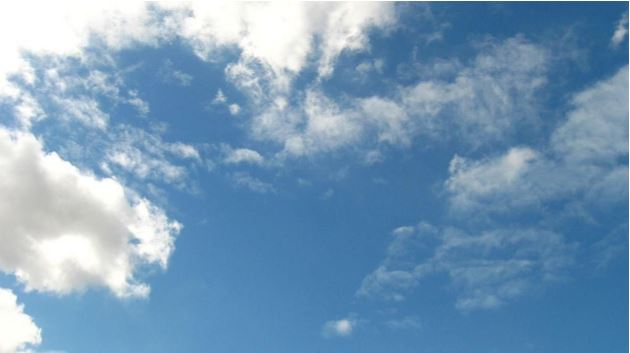
\includegraphics[scale=0.35]{images/sky.JPG}};
					
					\draw[thick] (-8.5,9) -- (-7.9,9);
					\draw[thick] (-8.5,9) -- (-8.5,11);
					\draw[->] (-8.5,11) -- (-8.15,11);
				}
				\onslide<3->{	
					\draw[blue] (-5.35,11.8) ellipse (0.05 and 0.09);		
					\draw[blue] (-5.35,12.25) ellipse (0.05 and 0.09);		
					\draw[blue] (-5.2,12.3) ellipse (0.05 and 0.09);				
					\draw[blue] (-5.4,12.5) ellipse (0.05 and 0.09);				
					\draw[blue] (-5.3,12.7) ellipse (0.05 and 0.09);				
					\draw[blue] (-5.1,13.1) ellipse (0.05 and 0.09);				
					\draw[blue] (-4.9,13.4) ellipse (0.05 and 0.09);				
					\draw[blue] (-4.85,13.65) ellipse (0.05 and 0.09);				
					\draw[blue] (-5.22,12.95) ellipse (0.05 and 0.09);	
					\draw[blue] (-5.16,12.65) ellipse (0.05 and 0.09);	
									
					\draw[blue] (-5.25,12) ellipse (0.05 and 0.09);		
					\draw[blue] (-5.05,12.25) ellipse (0.05 and 0.09);			
					\draw[blue] (-5,12.5) ellipse (0.05 and 0.09);			
					\draw[blue] (-5,12.8) ellipse (0.05 and 0.09);			
					\draw[blue] (-4.9,13) ellipse (0.05 and 0.09);			
					\draw[blue] (-4.8,12.6) ellipse (0.05 and 0.09);			
					%	\draw[blue] (-2.35,9.85) ellipse (0.05 and 0.09);			
				}
			\end{tikzpicture}
		\end{overlayarea}
		
		\column{0.5\textwidth}	
		\begin{overlayarea}{\textwidth}{\textheight}
			\begin{itemize}
				\justifying
				\onslide<1->{
					\item Suppose instead of starting with a blank (zero) image we start with an actual image.
					}	
				\onslide<3->{
					\item We focus on some layer and check the activations of the neurons 
					}	
				\onslide<4->{
					\item We want to change the image so that these neurons fire even more
					}	
								
			\end{itemize}
			
		\end{overlayarea}
	\end{columns}			
	
\end{frame}

%%%%%%%%%%%%%%%%%%%%%%%%%%%%%%%%%%%%%%%%%%%%%%%%%%%%%%%%%%%%%%%%%%%%%%%%%%%%%%%%%%%%%%%%%

\begin{frame}
\begin{columns}
	\column{0.5\textwidth}	
	
	\begin{overlayarea}{\textwidth}{\textheight}
		\begin{tikzpicture}
				
			\onslide<1->{
				\node[inner sep=0pt] (B) at (-4.7,12.5){
				%\begin{center}
\begin{tikzpicture}[scale=0.4,transform shape]

\pgfsetxvec{\pgfpoint{1cm}{0cm}}
\pgfsetyvec{\pgfpoint{0cm}{1cm}}
\pgfsetzvec{\pgfpoint{-.5cm}{-.866cm}}

\def\cuboid#1#2#3#4#5{
\begin{scope}
\edef\mycolor{#2}
\edef\depth{#3}
\edef\height{#4}
\edef\width{#5}
\draw[black,fill=\mycolor, fill opacity=0.4, text opacity=1] #1 -- ++(-\depth,0,0) -- ++(0,-\height,0) -- ++(\depth,0,0) -- cycle #1 -- ++(0,0,-\width) -- ++(0,-\height,0) -- ++(0,0,\width) -- cycle  #1 -- ++(-\depth,0,0) -- ++(0,0,-\width) -- ++(\depth,0,0) -- cycle;
\end{scope}
}

\def\cuboidlabel#1#2#3#4#5#6#7#8{
\begin{scope}
\edef\mycolor{#2}
\edef\depth{#3}
\edef\height{#4}
\edef\width{#5}
\edef\depthlabel{#6}
\edef\heightlabel{#7}
\edef\widthlabel{#8}
\draw[draw=none,fill=\mycolor, fill opacity=0.4, text opacity=1] #1 -- ++(-\depth,0,0) -- ++(0,-\height,0) -- ++(\depth,0,0) node[black,pos=0.5,below] {\tiny \depthlabel} -- cycle #1 -- ++(0,0,-\width) -- ++(0,-\height,0) node[black,pos=0.5,right] {\tiny \heightlabel} -- ++(0,0,\width)  node[black,pos=0.5,below,right] {\tiny \widthlabel} -- cycle  #1 -- ++(-\depth,0,0) -- ++(0,0,-\width) -- ++(\depth,0,0) -- cycle;
\end{scope}
}

\def\kernel#1#2#3#4#5#6{
\begin{scope}
\edef\mycolor{#2}
\edef\depth{#3}
\edef\height{#4}
\edef\width{#5}
\draw[black,fill=\mycolor, fill opacity=0.4, text opacity=1] #1 -- ++(-\depth,0,0) -- ++(0,-\height,0) -- ++(\depth,0,0) -- cycle #1 -- ++(0,0,-\width) -- ++(0,-\height,0) -- ++(0,0,\width) -- cycle  #1 -- ++(-\depth,0,0) -- ++(0,0,-\width) -- ++(\depth,0,0) -- cycle;

\draw[dotted] #1 -- #6 #1++(0,0,-\width) -- #6 #1++(0,-\height,0) -- #6 #1++(0,-\height,-\width) -- #6;

\end{scope}
}

\def\kernellabel#1#2#3#4#5#6#7#8#9{
%#6 is target pixel
\begin{scope}
\edef\mycolor{#2}
\edef\depth{#3}
\edef\height{#4}
\edef\width{#5}
\edef\depthlabel{#7}
\edef\heightlabel{#8}
\edef\widthlabel{#9}
\draw[draw=none,fill=\mycolor, fill opacity=0.4, text opacity=1] #1 -- ++(-\depth,0,0) -- ++(0,-\height,0) -- ++(\depth,0,0) -- cycle #1 -- ++(0,0,-\width) -- ++(0,-\height,0) node[pos=0.5,left] {\tiny \heightlabel} -- ++(0,0,\width)  node[pos=0.6,above] {\tiny \widthlabel} -- cycle  #1 -- ++(-\depth,0,0) -- ++(0,0,-\width) -- ++(\depth,0,0) -- cycle;

\draw[dotted] #1 -- #6 #1++(0,0,-\width) -- #6 #1++(0,-\height,0) -- #6 #1++(0,-\height,-\width) -- #6;

\end{scope}
}

%alexnet
\cuboidlabel{(0,0,0)}{gray}{0.03}{5.5}{5.5}{3}{227}{227}
\node (a) at (-0.015,-6.2,0) {\tiny Input};

\kernellabel{(0,-1,-1)}{blue}{0.03}{1.6}{1.6}{(1.7,-2,-2)}{3}{11}{11}


\cuboidlabel{(2,-0.5,-0.5)}{red}{0.6}{4.5}{4.5}{96}{55}{55}
\node (a) at (2-0.3,-0.5-4.5-0.7,-0.5) {\tiny Convolution};

\kernellabel{(2,-1.5,-1.5)}{blue}{0.6}{0.7}{0.7}{(3.7,-2.5,-2.5)}{96}{3}{3}


\cuboidlabel{(4,-1,-1)}{yellow}{0.6}{3.5}{3.5}{96}{27}{27}
\node (a) at (4-0.3,-1-3.5-0.7,-1) {\tiny MaxPooling};

%\kernellabel{(4,-2,-2)}{blue}{0.6}{1}{1}{(5.7,-3,-3)}{96}{5}{5}


\cuboidlabel{(6,-1.5,-1.5)}{red}{1}{3.3}{3.3}{256}{23}{23}
\node (a) at (6-0.5,-1.5-3.3-0.7,-1.5) {\tiny Convolution};

%\kernellabel{(6,-2.5,-2.5)}{blue}{1}{0.6}{0.6}{(7.7,-3.5,-3.5)}{256}{3}{3}


\cuboidlabel{(8,-2,-2)}{yellow}{1}{2.5}{2.5}{256}{11}{11}
\node (a) at (8-0.5,-2-2.5-0.7,-2) {\tiny MaxPooling};

\kernellabel{(8,-3,-3)}{blue}{1}{0.6}{0.6}{(9.7,-3.8,-3.8)}{256}{3}{3}


\cuboidlabel{(10,-2.5,-2.5)}{red}{1.3}{2.2}{2.2}{384}{9}{9}
\node (a) at (10-0.65,-2.5-2.2-0.7,-2.5) {\tiny Convolution};

\kernellabel{(10,-3.2,-3.2)}{blue}{1.3}{0.6}{0.6}{(11.5,-3.7,-3.7)}{384}{3}{3}


\cuboidlabel{(12,-3,-3)}{red}{1.3}{1.5}{1.5}{384}{7}{7}
\node (a) at (12-0.65,-3-1.5-0.7,-3) {\tiny Convolution};

\kernellabel{(12,-3.5,-3.5)}{blue}{1.3}{0.6}{0.6}{(13,-3.9,-3.9)}{384}{3}{3}


\cuboidlabel{(13.5,-3.5,-3.5)}{red}{1}{1}{1}{256}{5}{5}
\node (a) at (13.5-0.5,-3.5-1-0.7,-3.5) {\tiny Convolution};

\kernellabel{(13.5,-3.8,-3.8)}{blue}{1}{0.6}{0.6}{(14,-5.2,-5.2)}{256}{3}{3}

%\node (a) at (13.5-0.5+1,-6.7,-3.5) {\scriptsize $S=2$,$P=0$};
%\node (a) at (13.5-0.5+1,-7.2,-3.5) {\scriptsize Parameters: 0};


\cuboidlabel{(14.5,-5,-5)}{yellow}{1}{0.5}{0.5}{256}{2}{2}
\node (a) at (14.5-0.5,-5-0.5-0.7,-5) {\tiny MaxPooling};


%\draw[dotted,->] (14.5,-5,-5) -- (18,-0.7,0);
%\node (a) at (17.5,0,0) {\tiny dense};
%\cuboid{(18.5,3,0)}{red}{0.5}{7}{0}{256}{2}{2}
%\node (a) at (18.2,-4.5,0) {\tiny 4096};


%\draw[dotted,->] (18.5,-0.7,0) -- (19+0.5,-0.7,0) node[pos=0.5,above] {\tiny dense};
%\cuboid{(19.5+0.5,3,0)}{red}{0.5}{7}{0}{256}{2}{2}
%\node (a) at (19.2+0.5,-4.5,0) {\tiny 4096};
%
%
%\draw[dotted,->] (19.5+0.5,-0.7,0) -- (20+1,-0.7,0) node[pos=0.5,above] {\tiny dense};
%\cuboid{(20.5+1,2,0)}{red}{0.5}{5}{0}{256}{2}{2}
%\node (a) at (20.2+1,-3.5,0) {\tiny 1000};
%\cuboid{(20.5+1,1,0)}{green}{0.5}{0.5}{0}{256}{2}{2}
%\node (a) at (20.2+2,0.8,0) {\small Dumbell};

\end{tikzpicture}
%\end{center}


				};
			}	
				
			\onslide<1->{\node[inner sep=0pt] (A) at (-5,8.5) {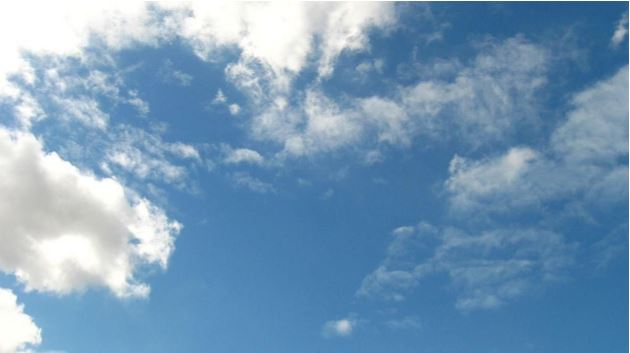
\includegraphics[scale=0.35]{images/sky.JPG}};
						
				\draw[thick] (-8.5,9) -- (-7.9,9);
				\draw[thick] (-8.5,9) -- (-8.5,11);
				\draw[->] (-8.5,11) -- (-8.15,11);
			}
			\onslide<1->{	
				\draw[blue] (-5.35,11.8) ellipse (0.05 and 0.09);		
				\draw[blue] (-5.35,12.25) ellipse (0.05 and 0.09);		
				\draw[blue] (-5.2,12.3) ellipse (0.05 and 0.09);				
				\draw[blue] (-5.4,12.5) ellipse (0.05 and 0.09);				
				\draw[blue] (-5.3,12.7) ellipse (0.05 and 0.09);				
				\draw[blue] (-5.1,13.1) ellipse (0.05 and 0.09);				
				\draw[blue] (-4.9,13.4) ellipse (0.05 and 0.09);				
				\draw[blue] (-4.85,13.65) ellipse (0.05 and 0.09);				
				\draw[blue] (-5.22,12.95) ellipse (0.05 and 0.09);	
				\draw[blue] (-5.16,12.65) ellipse (0.05 and 0.09);	
						
				\draw[blue] (-5.25,12) ellipse (0.05 and 0.09);		
				\draw[blue] (-5.05,12.25) ellipse (0.05 and 0.09);			
				\draw[blue] (-5,12.5) ellipse (0.05 and 0.09);			
				\draw[blue] (-5,12.8) ellipse (0.05 and 0.09);			
				\draw[blue] (-4.9,13) ellipse (0.05 and 0.09);			
				\draw[blue] (-4.8,12.6) ellipse (0.05 and 0.09);			
				
			}
			\onslide<3->{
				\draw[draw=blue,fill=cyan!20] (-5,12.8) ellipse (0.05 and 0.09);	
				\node at (-4.3,13.8) {$h_{ij}$};		
				\draw[->] (-4.9,12.8) -- (-4.4,13.7);
			}
		\end{tikzpicture}
	\end{overlayarea}
	\column{0.5\textwidth}	
	\begin{overlayarea}{\textwidth}{\textheight}
		\begin{itemize}
			\justifying
			\onslide<1->{
				\item How would we achieve this? %(boost activations of neurons)
			}	
			\onslide<2->{
				\item Suppose we want to boost the activation $h_{ij}$ (some neuron in some layer)
			}	
			\onslide<3->{
				\item We can formulate this as the following optimization problem
			}	
			\onslide<4->{
				\begin{align*}
					\max_{I} \mathscr{L}(I)   \\
					\mathscr{L}(I) = h^2_{ij} 
				\end{align*}
			}
			\vspace{-0.3cm}
			\onslide<5->{
				\item Consider a pixel $i_{mn}$ in the image 
						\begin{align*}
				      	\frac{\partial \mathscr{L}(I)}{\partial i_{mn}} = \frac{\partial \mathscr{L}(I)}{\partial h_{ij}}\frac{\partial h_{ij}}{\partial i_{mn}} 
					\end{align*}
			}
											
			\end{itemize}
						
		\end{overlayarea}
	\end{columns}			
					
\end{frame}

%%%%%%%%%%%%%%%%%%%%%%%%%%%%%%%%%%%%%%%%%%%%%%%%%%%%%%%%%%%%%%%%%%%%%%%%%%%%%%%%%%%%%%%%%
							
\begin{frame}
	\begin{columns}
		\column{0.5\textwidth}	
		\begin{overlayarea}{\textwidth}{\textheight}
			\begin{tikzpicture}
					
				\onslide<1->{
					\node[inner sep=0pt] (B) at (-4.7,12.5){
						%\begin{center}
\begin{tikzpicture}[scale=0.4,transform shape]

\pgfsetxvec{\pgfpoint{1cm}{0cm}}
\pgfsetyvec{\pgfpoint{0cm}{1cm}}
\pgfsetzvec{\pgfpoint{-.5cm}{-.866cm}}

\def\cuboid#1#2#3#4#5{
\begin{scope}
\edef\mycolor{#2}
\edef\depth{#3}
\edef\height{#4}
\edef\width{#5}
\draw[black,fill=\mycolor, fill opacity=0.4, text opacity=1] #1 -- ++(-\depth,0,0) -- ++(0,-\height,0) -- ++(\depth,0,0) -- cycle #1 -- ++(0,0,-\width) -- ++(0,-\height,0) -- ++(0,0,\width) -- cycle  #1 -- ++(-\depth,0,0) -- ++(0,0,-\width) -- ++(\depth,0,0) -- cycle;
\end{scope}
}

\def\cuboidlabel#1#2#3#4#5#6#7#8{
\begin{scope}
\edef\mycolor{#2}
\edef\depth{#3}
\edef\height{#4}
\edef\width{#5}
\edef\depthlabel{#6}
\edef\heightlabel{#7}
\edef\widthlabel{#8}
\draw[draw=none,fill=\mycolor, fill opacity=0.4, text opacity=1] #1 -- ++(-\depth,0,0) -- ++(0,-\height,0) -- ++(\depth,0,0) node[black,pos=0.5,below] {\tiny \depthlabel} -- cycle #1 -- ++(0,0,-\width) -- ++(0,-\height,0) node[black,pos=0.5,right] {\tiny \heightlabel} -- ++(0,0,\width)  node[black,pos=0.5,below,right] {\tiny \widthlabel} -- cycle  #1 -- ++(-\depth,0,0) -- ++(0,0,-\width) -- ++(\depth,0,0) -- cycle;
\end{scope}
}

\def\kernel#1#2#3#4#5#6{
\begin{scope}
\edef\mycolor{#2}
\edef\depth{#3}
\edef\height{#4}
\edef\width{#5}
\draw[black,fill=\mycolor, fill opacity=0.4, text opacity=1] #1 -- ++(-\depth,0,0) -- ++(0,-\height,0) -- ++(\depth,0,0) -- cycle #1 -- ++(0,0,-\width) -- ++(0,-\height,0) -- ++(0,0,\width) -- cycle  #1 -- ++(-\depth,0,0) -- ++(0,0,-\width) -- ++(\depth,0,0) -- cycle;

\draw[dotted] #1 -- #6 #1++(0,0,-\width) -- #6 #1++(0,-\height,0) -- #6 #1++(0,-\height,-\width) -- #6;

\end{scope}
}

\def\kernellabel#1#2#3#4#5#6#7#8#9{
%#6 is target pixel
\begin{scope}
\edef\mycolor{#2}
\edef\depth{#3}
\edef\height{#4}
\edef\width{#5}
\edef\depthlabel{#7}
\edef\heightlabel{#8}
\edef\widthlabel{#9}
\draw[draw=none,fill=\mycolor, fill opacity=0.4, text opacity=1] #1 -- ++(-\depth,0,0) -- ++(0,-\height,0) -- ++(\depth,0,0) -- cycle #1 -- ++(0,0,-\width) -- ++(0,-\height,0) node[pos=0.5,left] {\tiny \heightlabel} -- ++(0,0,\width)  node[pos=0.6,above] {\tiny \widthlabel} -- cycle  #1 -- ++(-\depth,0,0) -- ++(0,0,-\width) -- ++(\depth,0,0) -- cycle;

\draw[dotted] #1 -- #6 #1++(0,0,-\width) -- #6 #1++(0,-\height,0) -- #6 #1++(0,-\height,-\width) -- #6;

\end{scope}
}

%alexnet
\cuboidlabel{(0,0,0)}{gray}{0.03}{5.5}{5.5}{3}{227}{227}
\node (a) at (-0.015,-6.2,0) {\tiny Input};

\kernellabel{(0,-1,-1)}{blue}{0.03}{1.6}{1.6}{(1.7,-2,-2)}{3}{11}{11}


\cuboidlabel{(2,-0.5,-0.5)}{red}{0.6}{4.5}{4.5}{96}{55}{55}
\node (a) at (2-0.3,-0.5-4.5-0.7,-0.5) {\tiny Convolution};

\kernellabel{(2,-1.5,-1.5)}{blue}{0.6}{0.7}{0.7}{(3.7,-2.5,-2.5)}{96}{3}{3}


\cuboidlabel{(4,-1,-1)}{yellow}{0.6}{3.5}{3.5}{96}{27}{27}
\node (a) at (4-0.3,-1-3.5-0.7,-1) {\tiny MaxPooling};

%\kernellabel{(4,-2,-2)}{blue}{0.6}{1}{1}{(5.7,-3,-3)}{96}{5}{5}


\cuboidlabel{(6,-1.5,-1.5)}{red}{1}{3.3}{3.3}{256}{23}{23}
\node (a) at (6-0.5,-1.5-3.3-0.7,-1.5) {\tiny Convolution};

%\kernellabel{(6,-2.5,-2.5)}{blue}{1}{0.6}{0.6}{(7.7,-3.5,-3.5)}{256}{3}{3}


\cuboidlabel{(8,-2,-2)}{yellow}{1}{2.5}{2.5}{256}{11}{11}
\node (a) at (8-0.5,-2-2.5-0.7,-2) {\tiny MaxPooling};

\kernellabel{(8,-3,-3)}{blue}{1}{0.6}{0.6}{(9.7,-3.8,-3.8)}{256}{3}{3}


\cuboidlabel{(10,-2.5,-2.5)}{red}{1.3}{2.2}{2.2}{384}{9}{9}
\node (a) at (10-0.65,-2.5-2.2-0.7,-2.5) {\tiny Convolution};

\kernellabel{(10,-3.2,-3.2)}{blue}{1.3}{0.6}{0.6}{(11.5,-3.7,-3.7)}{384}{3}{3}


\cuboidlabel{(12,-3,-3)}{red}{1.3}{1.5}{1.5}{384}{7}{7}
\node (a) at (12-0.65,-3-1.5-0.7,-3) {\tiny Convolution};

\kernellabel{(12,-3.5,-3.5)}{blue}{1.3}{0.6}{0.6}{(13,-3.9,-3.9)}{384}{3}{3}


\cuboidlabel{(13.5,-3.5,-3.5)}{red}{1}{1}{1}{256}{5}{5}
\node (a) at (13.5-0.5,-3.5-1-0.7,-3.5) {\tiny Convolution};

\kernellabel{(13.5,-3.8,-3.8)}{blue}{1}{0.6}{0.6}{(14,-5.2,-5.2)}{256}{3}{3}

%\node (a) at (13.5-0.5+1,-6.7,-3.5) {\scriptsize $S=2$,$P=0$};
%\node (a) at (13.5-0.5+1,-7.2,-3.5) {\scriptsize Parameters: 0};


\cuboidlabel{(14.5,-5,-5)}{yellow}{1}{0.5}{0.5}{256}{2}{2}
\node (a) at (14.5-0.5,-5-0.5-0.7,-5) {\tiny MaxPooling};


%\draw[dotted,->] (14.5,-5,-5) -- (18,-0.7,0);
%\node (a) at (17.5,0,0) {\tiny dense};
%\cuboid{(18.5,3,0)}{red}{0.5}{7}{0}{256}{2}{2}
%\node (a) at (18.2,-4.5,0) {\tiny 4096};


%\draw[dotted,->] (18.5,-0.7,0) -- (19+0.5,-0.7,0) node[pos=0.5,above] {\tiny dense};
%\cuboid{(19.5+0.5,3,0)}{red}{0.5}{7}{0}{256}{2}{2}
%\node (a) at (19.2+0.5,-4.5,0) {\tiny 4096};
%
%
%\draw[dotted,->] (19.5+0.5,-0.7,0) -- (20+1,-0.7,0) node[pos=0.5,above] {\tiny dense};
%\cuboid{(20.5+1,2,0)}{red}{0.5}{5}{0}{256}{2}{2}
%\node (a) at (20.2+1,-3.5,0) {\tiny 1000};
%\cuboid{(20.5+1,1,0)}{green}{0.5}{0.5}{0}{256}{2}{2}
%\node (a) at (20.2+2,0.8,0) {\small Dumbell};

\end{tikzpicture}
%\end{center}


					};
				}	
					
				\onslide<1->{\node[inner sep=0pt] (A) at (-5,8.5) {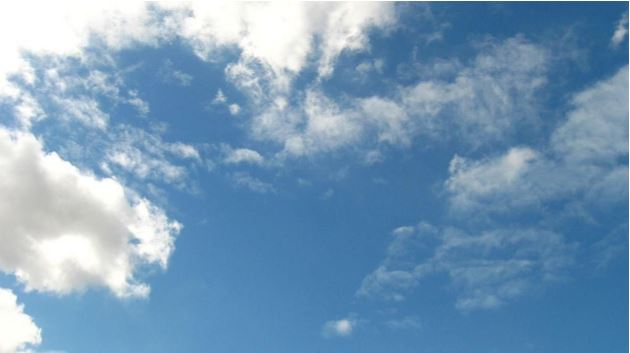
\includegraphics[scale=0.35]{images/sky.JPG}};
							
					\draw[thick] (-8.5,9) -- (-7.9,9);
					\draw[thick] (-8.5,9) -- (-8.5,11);
					\draw[->] (-8.5,11) -- (-8.15,11);
				}
				\onslide<1->{	
					\draw[blue] (-5.35,11.8) ellipse (0.05 and 0.09);		
					\draw[blue] (-5.35,12.25) ellipse (0.05 and 0.09);		
					\draw[blue] (-5.2,12.3) ellipse (0.05 and 0.09);				
					\draw[blue] (-5.4,12.5) ellipse (0.05 and 0.09);				
					\draw[blue] (-5.3,12.7) ellipse (0.05 and 0.09);				
					\draw[blue] (-5.1,13.1) ellipse (0.05 and 0.09);				
					\draw[blue] (-4.9,13.4) ellipse (0.05 and 0.09);				
					\draw[blue] (-4.85,13.65) ellipse (0.05 and 0.09);				
					\draw[blue] (-5.22,12.95) ellipse (0.05 and 0.09);	
					\draw[blue] (-5.16,12.65) ellipse (0.05 and 0.09);	
							
					\draw[blue] (-5.25,12) ellipse (0.05 and 0.09);		
					\draw[blue] (-5.05,12.25) ellipse (0.05 and 0.09);			
					\draw[blue] (-5,12.5) ellipse (0.05 and 0.09);			
					\draw[blue] (-5,12.8) ellipse (0.05 and 0.09);			
					\draw[blue] (-4.9,13) ellipse (0.05 and 0.09);			
					\draw[blue] (-4.8,12.6) ellipse (0.05 and 0.09);			
					\onslide<2->{	\draw[draw=blue,fill=cyan!50] (-5,12.8) ellipse (0.05 and 0.09);	
						\node at (-4.3,13.9) {$h_{ij}$};		
						\draw[->]  (-4.4,13.7) --  (-4.9,12.8);
					}	
				}
				\onslide<2->{
					\draw[draw=blue,fill=cyan!20] (-5,12.8) ellipse (0.05 and 0.09);	
						
				}
			\end{tikzpicture}
		\end{overlayarea}
		\column{0.5\textwidth}	
		\begin{overlayarea}{\textwidth}{\textheight}
			\begin{itemize}
				\justifying
				\onslide<1->{
					\item Once the image is updated $\Big(i_{mn} = i_{mn} + \frac{\partial \mathscr{L}(I)}{\partial i_{mn}}\Big)$ we feed it back to the network
				}	
				\onslide<2->{
					\item This time the target neurons should fire even more (because we have precisely modified the image to achieve this)
				}	
				\onslide<3->{
					\item Doing this iteratively would make the image more and more like the patterns that cause the neuron to fire
				}	
				\onslide<4->{
					\item Let us run this algorithm
				}	
								
								
			\end{itemize}
						
		\end{overlayarea}
	\end{columns}			
		
\end{frame}

%%%%%%%%%%%%%%%%%%%%%%%%%%%%%%%%%%%%%%%%%%%%%%%%%%%%%%%%%%%%%%%%%%%%%%%%%%%%%%%%%%%%%%%%%

\begin{frame}
	\foreach \x in {0,...,99}
	{
		\only<\x>{
			\centering
			\includegraphics[scale=0.4]{images/Sky-Frames/0_\x.jpg}
		}
	}
\end{frame}

%%%%%%%%%%%%%%%%%%%%%%%%%%%%%%%%%%%%%%%%%%%%%%%%%%%%%%%%%%%%%%%%%%%%%%%%%%%%%%%%%%%%%%%%%

\begin{frame}
	\foreach \x in {0,...,99}
	{
		\only<\x>{
			\centering
			\includegraphics[scale=0.4]{images/Monsoon-Frames/0_\x.jpg}
		}
	}
\end{frame}

%%%%%%%%%%%%%%%%%%%%%%%%%%%%%%%%%%%%%%%%%%%%%%%%%%%%%%%%%%%%%%%%%%%%%%%%%%%%%%%%%%%%%%%%%

\begin{frame}
	\foreach \x in {0,...,99}
	{
		\only<\x>{
			\centering
			\includegraphics[scale=0.33]{images/Leonardo-frames/0_\x.jpg}
		}
	}
\end{frame}

%%%%%%%%%%%%%%%%%%%%%%%%%%%%%%%%%%%%%%%%%%%%%%%%%%%%%%%%%%%%%%%%%%%%%%%%%%%%%%%%%%%%%%%%%

\begin{frame}
\begin{columns}
	\column{0.45\textwidth}	
	
	\begin{overlayarea}{\textwidth}{\textheight}
		\begin{tikzpicture}
				
			\onslide<1->{
				\node[inner sep=0pt] (B) at (-4.7,12.5){
					%\begin{center}
\begin{tikzpicture}[scale=0.4,transform shape]

\pgfsetxvec{\pgfpoint{1cm}{0cm}}
\pgfsetyvec{\pgfpoint{0cm}{1cm}}
\pgfsetzvec{\pgfpoint{-.5cm}{-.866cm}}

\def\cuboid#1#2#3#4#5{
\begin{scope}
\edef\mycolor{#2}
\edef\depth{#3}
\edef\height{#4}
\edef\width{#5}
\draw[black,fill=\mycolor, fill opacity=0.4, text opacity=1] #1 -- ++(-\depth,0,0) -- ++(0,-\height,0) -- ++(\depth,0,0) -- cycle #1 -- ++(0,0,-\width) -- ++(0,-\height,0) -- ++(0,0,\width) -- cycle  #1 -- ++(-\depth,0,0) -- ++(0,0,-\width) -- ++(\depth,0,0) -- cycle;
\end{scope}
}

\def\cuboidlabel#1#2#3#4#5#6#7#8{
\begin{scope}
\edef\mycolor{#2}
\edef\depth{#3}
\edef\height{#4}
\edef\width{#5}
\edef\depthlabel{#6}
\edef\heightlabel{#7}
\edef\widthlabel{#8}
\draw[draw=none,fill=\mycolor, fill opacity=0.4, text opacity=1] #1 -- ++(-\depth,0,0) -- ++(0,-\height,0) -- ++(\depth,0,0) node[black,pos=0.5,below] {\tiny \depthlabel} -- cycle #1 -- ++(0,0,-\width) -- ++(0,-\height,0) node[black,pos=0.5,right] {\tiny \heightlabel} -- ++(0,0,\width)  node[black,pos=0.5,below,right] {\tiny \widthlabel} -- cycle  #1 -- ++(-\depth,0,0) -- ++(0,0,-\width) -- ++(\depth,0,0) -- cycle;
\end{scope}
}

\def\kernel#1#2#3#4#5#6{
\begin{scope}
\edef\mycolor{#2}
\edef\depth{#3}
\edef\height{#4}
\edef\width{#5}
\draw[black,fill=\mycolor, fill opacity=0.4, text opacity=1] #1 -- ++(-\depth,0,0) -- ++(0,-\height,0) -- ++(\depth,0,0) -- cycle #1 -- ++(0,0,-\width) -- ++(0,-\height,0) -- ++(0,0,\width) -- cycle  #1 -- ++(-\depth,0,0) -- ++(0,0,-\width) -- ++(\depth,0,0) -- cycle;

\draw[dotted] #1 -- #6 #1++(0,0,-\width) -- #6 #1++(0,-\height,0) -- #6 #1++(0,-\height,-\width) -- #6;

\end{scope}
}

\def\kernellabel#1#2#3#4#5#6#7#8#9{
%#6 is target pixel
\begin{scope}
\edef\mycolor{#2}
\edef\depth{#3}
\edef\height{#4}
\edef\width{#5}
\edef\depthlabel{#7}
\edef\heightlabel{#8}
\edef\widthlabel{#9}
\draw[draw=none,fill=\mycolor, fill opacity=0.4, text opacity=1] #1 -- ++(-\depth,0,0) -- ++(0,-\height,0) -- ++(\depth,0,0) -- cycle #1 -- ++(0,0,-\width) -- ++(0,-\height,0) node[pos=0.5,left] {\tiny \heightlabel} -- ++(0,0,\width)  node[pos=0.6,above] {\tiny \widthlabel} -- cycle  #1 -- ++(-\depth,0,0) -- ++(0,0,-\width) -- ++(\depth,0,0) -- cycle;

\draw[dotted] #1 -- #6 #1++(0,0,-\width) -- #6 #1++(0,-\height,0) -- #6 #1++(0,-\height,-\width) -- #6;

\end{scope}
}

%alexnet
\cuboidlabel{(0,0,0)}{gray}{0.03}{5.5}{5.5}{3}{227}{227}
\node (a) at (-0.015,-6.2,0) {\tiny Input};

\kernellabel{(0,-1,-1)}{blue}{0.03}{1.6}{1.6}{(1.7,-2,-2)}{3}{11}{11}


\cuboidlabel{(2,-0.5,-0.5)}{red}{0.6}{4.5}{4.5}{96}{55}{55}
\node (a) at (2-0.3,-0.5-4.5-0.7,-0.5) {\tiny Convolution};

\kernellabel{(2,-1.5,-1.5)}{blue}{0.6}{0.7}{0.7}{(3.7,-2.5,-2.5)}{96}{3}{3}


\cuboidlabel{(4,-1,-1)}{yellow}{0.6}{3.5}{3.5}{96}{27}{27}
\node (a) at (4-0.3,-1-3.5-0.7,-1) {\tiny MaxPooling};

%\kernellabel{(4,-2,-2)}{blue}{0.6}{1}{1}{(5.7,-3,-3)}{96}{5}{5}


\cuboidlabel{(6,-1.5,-1.5)}{red}{1}{3.3}{3.3}{256}{23}{23}
\node (a) at (6-0.5,-1.5-3.3-0.7,-1.5) {\tiny Convolution};

%\kernellabel{(6,-2.5,-2.5)}{blue}{1}{0.6}{0.6}{(7.7,-3.5,-3.5)}{256}{3}{3}


\cuboidlabel{(8,-2,-2)}{yellow}{1}{2.5}{2.5}{256}{11}{11}
\node (a) at (8-0.5,-2-2.5-0.7,-2) {\tiny MaxPooling};

\kernellabel{(8,-3,-3)}{blue}{1}{0.6}{0.6}{(9.7,-3.8,-3.8)}{256}{3}{3}


\cuboidlabel{(10,-2.5,-2.5)}{red}{1.3}{2.2}{2.2}{384}{9}{9}
\node (a) at (10-0.65,-2.5-2.2-0.7,-2.5) {\tiny Convolution};

\kernellabel{(10,-3.2,-3.2)}{blue}{1.3}{0.6}{0.6}{(11.5,-3.7,-3.7)}{384}{3}{3}


\cuboidlabel{(12,-3,-3)}{red}{1.3}{1.5}{1.5}{384}{7}{7}
\node (a) at (12-0.65,-3-1.5-0.7,-3) {\tiny Convolution};

\kernellabel{(12,-3.5,-3.5)}{blue}{1.3}{0.6}{0.6}{(13,-3.9,-3.9)}{384}{3}{3}


\cuboidlabel{(13.5,-3.5,-3.5)}{red}{1}{1}{1}{256}{5}{5}
\node (a) at (13.5-0.5,-3.5-1-0.7,-3.5) {\tiny Convolution};

\kernellabel{(13.5,-3.8,-3.8)}{blue}{1}{0.6}{0.6}{(14,-5.2,-5.2)}{256}{3}{3}

%\node (a) at (13.5-0.5+1,-6.7,-3.5) {\scriptsize $S=2$,$P=0$};
%\node (a) at (13.5-0.5+1,-7.2,-3.5) {\scriptsize Parameters: 0};


\cuboidlabel{(14.5,-5,-5)}{yellow}{1}{0.5}{0.5}{256}{2}{2}
\node (a) at (14.5-0.5,-5-0.5-0.7,-5) {\tiny MaxPooling};


%\draw[dotted,->] (14.5,-5,-5) -- (18,-0.7,0);
%\node (a) at (17.5,0,0) {\tiny dense};
%\cuboid{(18.5,3,0)}{red}{0.5}{7}{0}{256}{2}{2}
%\node (a) at (18.2,-4.5,0) {\tiny 4096};


%\draw[dotted,->] (18.5,-0.7,0) -- (19+0.5,-0.7,0) node[pos=0.5,above] {\tiny dense};
%\cuboid{(19.5+0.5,3,0)}{red}{0.5}{7}{0}{256}{2}{2}
%\node (a) at (19.2+0.5,-4.5,0) {\tiny 4096};
%
%
%\draw[dotted,->] (19.5+0.5,-0.7,0) -- (20+1,-0.7,0) node[pos=0.5,above] {\tiny dense};
%\cuboid{(20.5+1,2,0)}{red}{0.5}{5}{0}{256}{2}{2}
%\node (a) at (20.2+1,-3.5,0) {\tiny 1000};
%\cuboid{(20.5+1,1,0)}{green}{0.5}{0.5}{0}{256}{2}{2}
%\node (a) at (20.2+2,0.8,0) {\small Dumbell};

\end{tikzpicture}
%\end{center}


				};}	
				
			\onslide<1->{\node[inner sep=0pt] (A) at (-5,8.5) {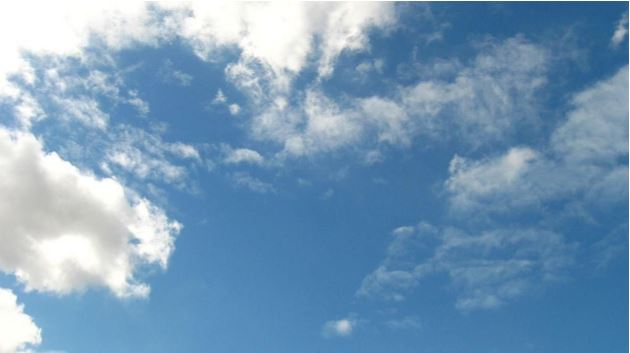
\includegraphics[scale=0.35]{images/sky.JPG}};
						
				\draw[thick] (-8.5,9) -- (-7.9,9);
				\draw[thick] (-8.5,9) -- (-8.5,11);
				\draw[->] (-8.5,11) -- (-8.15,11);
			}
			\onslide<1->{	
				\draw[draw=blue,fill=myblue1] (-5.35,11.8) ellipse (0.05 and 0.09);		
				\draw[draw=blue,fill=myblue2] (-5.35,12.25) ellipse (0.05 and 0.09);		
				\draw[draw=blue,fill=myblue3] (-5.2,12.3) ellipse (0.05 and 0.09);				
				\draw[draw=blue,fill=myblue4] (-5.4,12.5) ellipse (0.05 and 0.09);				
				\draw[draw=blue,fill=myblue1] (-5.3,12.7) ellipse (0.05 and 0.09);				
				\draw[draw=blue,fill=myblue2] (-5.1,13.1) ellipse (0.05 and 0.09);				
				\draw[draw=blue,fill=myblue3] (-4.9,13.4) ellipse (0.05 and 0.09);				
				\draw[draw=blue,fill=myblue4] (-4.85,13.65) ellipse (0.05 and 0.09);			
				\draw[draw=blue,fill=myblue1] (-5.22,12.95) ellipse (0.05 and 0.09);	
				\draw[draw=blue,fill=myblue2] (-5.16,12.65) ellipse (0.05 and 0.09);	
						
				\draw[draw=blue,fill=myblue3] (-5.25,12) ellipse (0.05 and 0.09);		
				\draw[draw=blue,fill=myblue4] (-5.05,12.25) ellipse (0.05 and 0.09);			
				\draw[draw=blue,fill=myblue1] (-5,12.5) ellipse (0.05 and 0.09);			
				\draw[draw=blue,fill=myblue2] (-5,12.8) ellipse (0.05 and 0.09);			
				\draw[draw=blue,fill=myblue3] (-4.9,13) ellipse (0.05 and 0.09);			
				\draw[draw=blue,fill=myblue4] (-4.8,12.6) ellipse (0.05 and 0.09);			
						
			}
				
		\end{tikzpicture}
	\end{overlayarea}
	
			
			
	\column{0.55\textwidth}	
	\begin{overlayarea}{\textwidth}{\textheight}
		\begin{itemize}
			\justifying
			\onslide<1->{
				\item So what exactly is happening here?	
			}	
			\onslide<2->{
				\item The network has been trained to detect certain patterns (dogs, cat, birds etc.) which appear frequently in the ImageNet data
			}	
			\onslide<3->{
				\item It starts seeing these patterns even when they hardly exist
			}	
			\onslide<4->{
				\item \it{If a cloud looks a little bit like a bird, the network will make it look more like a bird. This in turn will make the network recognize the bird even more strongly on the next pass and so forth, until a highly detailed bird appears seemingly out of nowhere. - Google$^*$\footnotetext{$^*$\url{research.googleblog.com/2015/06/inceptionism-}\\ \url{going-deeper-into-neural.html}}}}	
			      				
			      				
		\end{itemize}
					
	\end{overlayarea}
	\end{columns}			
		
\end{frame}
